\documentclass[11pt, oneside]{article} 
\usepackage{geometry}
\geometry{letterpaper} 
\usepackage{graphicx}
	
\usepackage{amssymb}
\usepackage{amsmath}
\usepackage{parskip}
\usepackage{color}
\usepackage{hyperref}

\graphicspath{{/Users/telliott_admin/Dropbox/Tex/png/}}
% \begin{center} 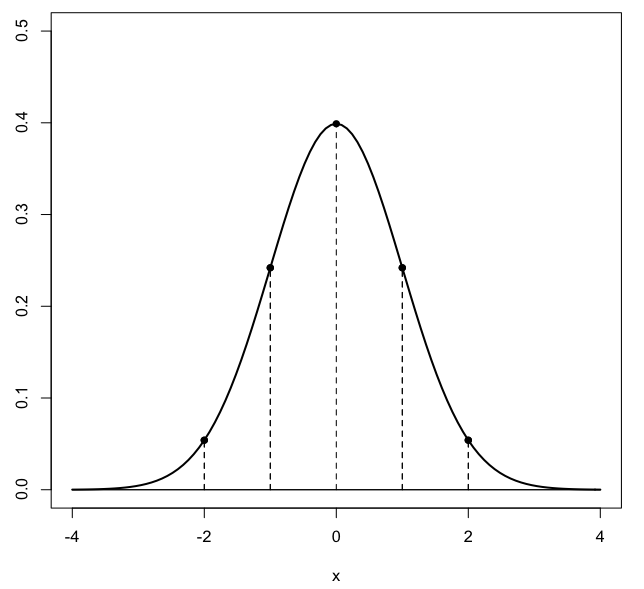
\includegraphics [scale=0.4] {gauss3.png} \end{center}

\title{Quadrature of the Parabola}
\date{}

\begin{document}
\maketitle
\Large
\begin{center} 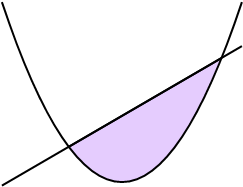
\includegraphics [scale=0.35] {Parabolic_Segment.png} \end{center}
Consider a parabolic segment, the area bounded by a straight line drawn between two points on a parabola, and the parabola itself. Draw the tangent parallel to the line segment we already have.

\begin{center} 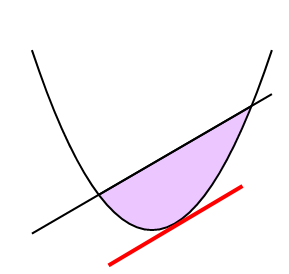
\includegraphics [scale=0.40] {Parabolic_Segment2.png} \end{center}

We will show first that the x-coordinate of the point of tangency is exactly half-way (on the x-axis) between the two points at which the line segment intersects the parabola.
\begin{center} 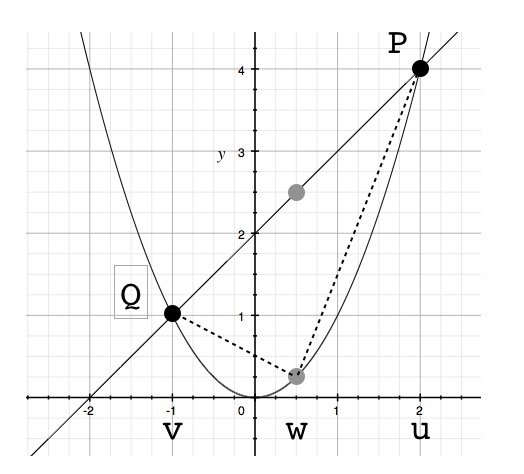
\includegraphics [scale=0.40] {para_tri2.png} \end{center}
Let $P$ be $(u,au^2)$ and $Q$ be $(v,av^2)$ so the slope of the line connecting them is 
\[ \frac{\Delta y}{\Delta x} = \frac{au^2 - av^2}{u - v} = a(u + v) \]
This is equal to the slope of the tangent at $x = w$, which by simple calculus is $2aw$ so:
\[ 2aw = a(u + v) \]
$w$ is the \emph{average} of $u$ and $v$ and lies half-way between them:
\[ w = \frac{1}{2}(u + v) = v + \frac{1}{2}(u - v) \]

Draw the triangle connecting our three points.
\begin{center} 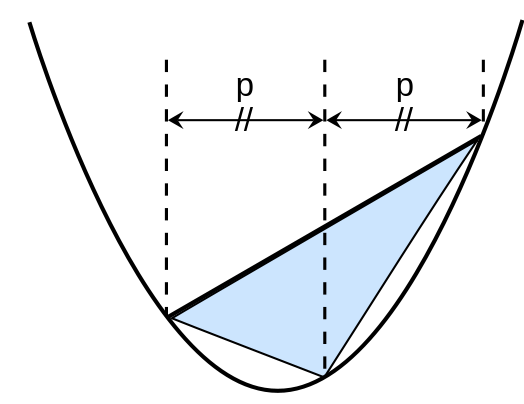
\includegraphics [scale=0.3] {para_tri4.png} \end{center}
The two halves of the blue triangle (divided by the longest of the three dotted vertical lines), have equal area.  They share the same (vertical) "base", and their "heights" in the x-direction are also equal, as we just showed (usually a "base" is horizontal, here all bases are vertical and all "heights" horizontal).

Suppose we now repeat the process, drawing two new triangles with their apexes at the points where the tangents are parallel to the base (light green).
\begin{center} 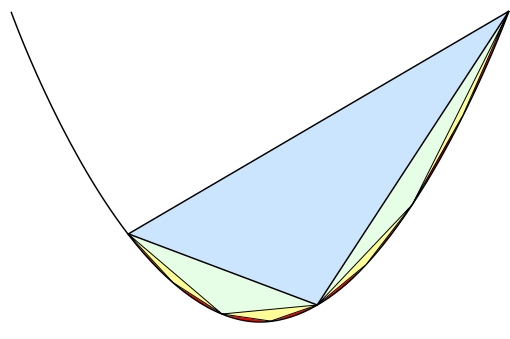
\includegraphics [scale=0.3] {para_tri5.png} \end{center}

The x-coordinate of the point on the right will be half way between $w$ and $u$.  The horizontal height of that triangle will be decreased by one-half, compared to the one in blue.  What about its base?
\begin{center} 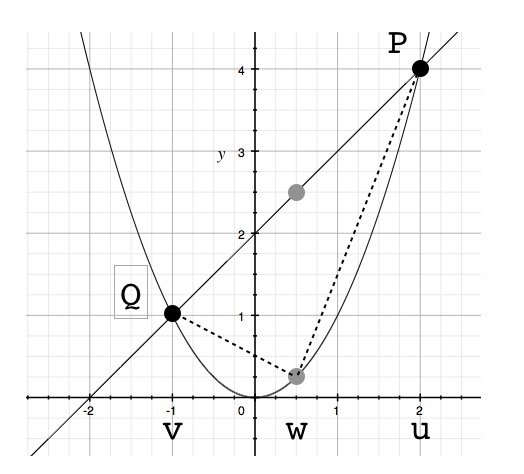
\includegraphics [scale=0.40] {para_tri2.png} \end{center}

First we calculate the original base.  The point half-way between $P$ and $Q$ has y-coordinate $(au^2 + av^2)/2$.  The length of the vertical down to the point $(w,aw^2)$ is
\[ \frac{1}{2}(au^2 + av^2) - aw^2 \]
\[ = \frac{1}{2}(au^2 + av^2) - a\ [ \frac{u + v}{2} \ ]^2 \]
\[ = \frac{a}{4} \ [ 2u^2 + 2v^2 - (u^2 + v^2 + 2uv) \ ] \]
\[ = \frac{a}{4} (u-v)^2 \]

Let $z$ be the x-coordinate of the point halfway between $w$ and $u$.  

\begin{center} 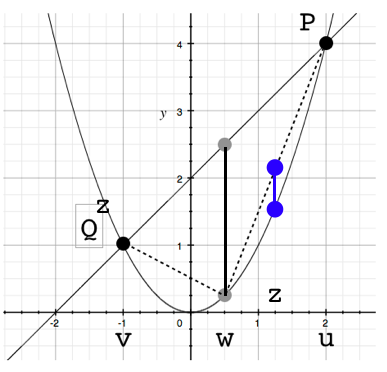
\includegraphics [scale=0.40] {para_tri2b.png} \end{center}

By analogy to the calculation we just did, the vertical distance for the new light green triangles is
\[ = \frac{a}{4} (u-w)^2 \]
and the ratio of the smaller to the larger distance (the ratio of the bases for the blue and green triangles) is
\[ \frac{(u - v)^2}{(u - w)^2} \]
\[ = \frac{(u - v)^2}{(u - 1/2(u+v))^2} \]
\[ = \frac{(u - v)^2}{[ (u - v)/2 \ ]^2} = 4 \]
In other words, each of the two small green triangles has a height $1/2$ that of the original blue one, with a base that is $1/4$, so the total area is $1/8$ of the original.  

However, there are two green triangles, thus the additional area obtained from the two green triangles is one-quarter that of the blue one.

Our new estimate for the area bounded by the parabola and the line is the area of the blue triangle plus the two green ones, which is
\[ A + \frac{1}{4} A \]
Repeating the process yields
\[ A + \frac{1}{4} A + (\frac{1}{4})^2 A  + \dots \]
\[ = A  \ [ \ 1 + \frac{1}{4}  + (\frac{1}{4})^2   + \dots \ ] \]
\[ = A (1 + \frac{1}{3}) = \frac{4}{3} A \]

\begin{center} 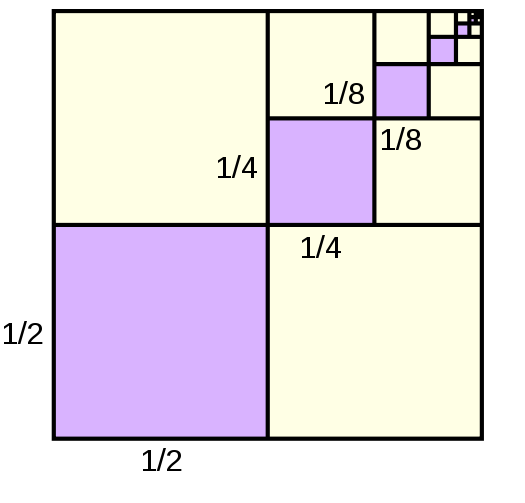
\includegraphics [scale=0.4] {para_series_sum.png} \end{center}



\end{document}  